\documentclass[a4paper,10pt]{article}


%%%%%%%%%%%%%%%%%%%%%%%%%%%%%%%%%%%%%%%%%%%%%%%%
% Set up basic variables for the Homework

% Enter your personal data here
\newcommand{\name}{Mustermann}
\newcommand{\firstname}{Max}
\newcommand{\mail}{max.mustermann@student.tuwien.ac.at}
\newcommand{\registration}{1345678}

% Set exercise name
\newcommand{\exercise}{Demo}

%%%%%%%%%%%%%%%%%%%%%%%%%%%%%%%%%%%%%%%%%%%%%%%%


% Set the language to German
\usepackage[english]{babel}
\usepackage[utf8]{inputenc}

% Enable colouring
\usepackage[table]{xcolor}  

% Set layout
\usepackage[a4paper, portrait, margin=1.5in, left=1in, right=1in, headheight=33pt]{geometry}

% Enable a fancy header for your convenience
\usepackage{fancyhdr}

\pagestyle{fancy}
\fancyhf{}
\rhead{\firstname\ \name\\
\small{\registration \\
\mail}}
\lhead{\exercise}
\rfoot{Page \thepage}

% Set up formating without slide in first line
\usepackage{parskip}
\usepackage{amssymb}
\usepackage{amsmath}

% Enable hyperlinks
\usepackage{hyperref}

%%%%%%%%%%%%%%%%%%%%%%%%%%%%%
% Set code background colour
\definecolor{light-gray}{gray}{0.95}
%%%%%%%%%%%%%%%%%%%%%%%%%%%%%

% Set up code highlighting
\usepackage{minted}
\usemintedstyle{manni}
\setminted{frame=lines, framesep=2mm, baselinestretch=1.2, fontsize=\footnotesize, linenos, bgcolor=light-gray}
\setmintedinline{frame=none, framesep=2mm, baselinestretch=0, fontsize=\footnotesize, linenos, bgcolor=white}

% Add an arrowlist
\usepackage{enumitem}
\newlist{arrowlist}{itemize}{1}
\setlist[arrowlist]{label=$\rightarrow$}

% Enable graph drawing
\usepackage{tikz}


%%%%%%%%%%%%%%%%%%%%%%%%%%%%%%%%%%%%%%%%%%%%%%%%%%
%%%%%%          DOCUMENT GOES HERE          %%%%%%
%%%%%%%%%%%%%%%%%%%%%%%%%%%%%%%%%%%%%%%%%%%%%%%%%%


\begin{document}

\section*{Demo section}
Demo document

\begin{minted}{java}

// This is a Java comment
String test = "Test!";
System.out.println(test);

if (true) {
	Test test1 = new Test();
	test1.testit();
}
\end{minted}

This is an example list:

\begin{arrowlist}
\item An example
\item Another example
\end{arrowlist}

\section*{Section 2 - Graphs}
This is a demo graph.

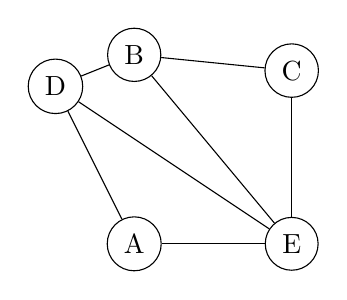
\begin{tikzpicture}[scale=2]
	% Nodes start here
	\node (A) at (1,0) [circle,draw] {A};
	\node (B) at (1,1.2) [circle,draw] {B};
	\node (C) at (2,1.1) [circle,draw] {C};
	\node (D) at (0.5,1) [circle,draw] {D};
	\node (E) at (2,0) [circle,draw] {E};

	% Lines start here
	\draw[-] (B) to (D);
	\draw[-] (A) to (D);
	\draw[-] (E) to (D);
	\draw[-] (E) to (B);
	\draw[-] (E) to (A);
	\draw[-] (E) to (C);
	\draw[-] (C) to (B);

\end{tikzpicture}

\section*{Installation}
All necessary packages should be installed automagically.\\
The package \texttt{minted} requires Python, which can be installed from \href{https://www.python.org/downloads/}{the official download page}. Make sure to enable to have the \texttt{path} variable set during installation. You then need to install Pygments using the command line:
\mint{bash}|pip3 install Pygments|
Lastly you need to add the \texttt{--shell-escape} flag to the \LaTeX command of your build environment.

\end{document}